\documentclass[12pt]{article}
\newif\ifanswer\answertrue%\answerfalse% comment out to show/hide answers
\usepackage{../preamble3}% preamble always after \newif\ifanswer
%\pagenumbering{gobble}
\title{Art Of Problem Solving - AMC 10 \\ July 17, 2021}
\author{Patrick \& James Toche}
\date{Revised:~\today}

\begin{document}
\maketitle
\begin{minipage}{\textwidth}
\begin{abstract}\setlength{\parindent}{0pt}%
Notes on the AMC-10 Course by Art Of Problem Solving (AOPS).
Copyright restrictions may apply. Written for personal use. 
Please report typos and errors over at \url{https://github.com/ptoche/Math/tree/master/aops}. 
\end{abstract}
\end{minipage}

\thispagestyle{empty}
\clearpage


%%%%%%%%%%%%%%%%%%%%%%%%%%%%%%%%%%%%%%%%%%%%%%%%%%%%%%%%%%%%%%%%%%%%%%%%
\subsection*{1.}

\nopagebreak

In quadrilateral $ABCD$, $AB = 5$, $BC = 17$, $CD = 5$, $DA = 9$, and $BD$ is an integer. What is $BD$?

\begin{center}
  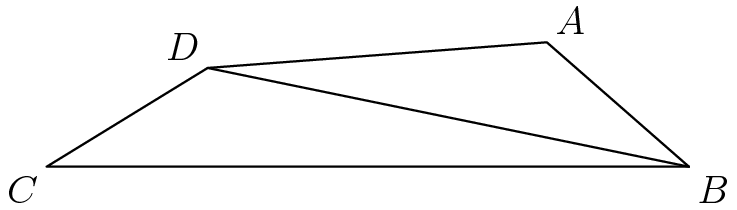
\includegraphics[height=3cm,page=1]{2021-07-17-homework-01}
\end{center}

\fbox{(A) $11$ \quad (B) $12$ \quad (C) $13$ \quad (D) $14$ \quad (E) $15$}

\begin{answer}
\begin{align*}
x
\end{align*}
\begin{empheq}[box={\mathbox[colback=white]}]{equation*}
    x
\end{empheq} 
\end{answer}
%%%%%%%%%%%%%%%%%%%%%%%%%%%%%%%%%%%%%%%%%%%%%%%%%%%%%%%%%%%%%%%%%%%%%%%%

\iftoggle{showAnswers}{\newpage}

%%%%%%%%%%%%%%%%%%%%%%%%%%%%%%%%%%%%%%%%%%%%%%%%%%%%%%%%%%%%%%%%%%%%%%%%
\subsection*{2.}

\nopagebreak

Rectangle $ABCD$ has $AB = 4$ and $BC = 3$. Segment $\overline{EF}$ is constructed through $B$ so that $\overline{EF} \perp \overline{DB}$, and $A$ and $C$ lie on $\overline{DE}$ and $\overline{DF}$, respectively. What is $EF$?

\fbox{(A) $9$ \quad (B) $10$ \quad (C) $\frac{125}{12}$ \quad (D) $\frac{103}{9}$ \quad (E) $12$}

\begin{answer}
\begin{align*}
x
\end{align*}
\begin{empheq}[box={\mathbox[colback=white]}]{equation*}
    x
\end{empheq} 
\end{answer}
%%%%%%%%%%%%%%%%%%%%%%%%%%%%%%%%%%%%%%%%%%%%%%%%%%%%%%%%%%%%%%%%%%%%%%%%

\iftoggle{showAnswers}{\newpage}

%%%%%%%%%%%%%%%%%%%%%%%%%%%%%%%%%%%%%%%%%%%%%%%%%%%%%%%%%%%%%%%%%%%%%%%%
\subsection*{3.}

\nopagebreak

Points $A$, $B$, $C$, $D$, $E$, and $F$ lie, in that order, on $\overline{AF}$, dividing it into five segments, each of length 1. Point $G$ is not on line $AF$. Point $H$ lies on $\overline{GD}$, and point $J$ lies on $\overline{GF}$. The line segments $\overline{HC}$, $\overline{JE}$, and $\overline{AG}$ are parallel. Find $HC/JE$.

\begin{center}
  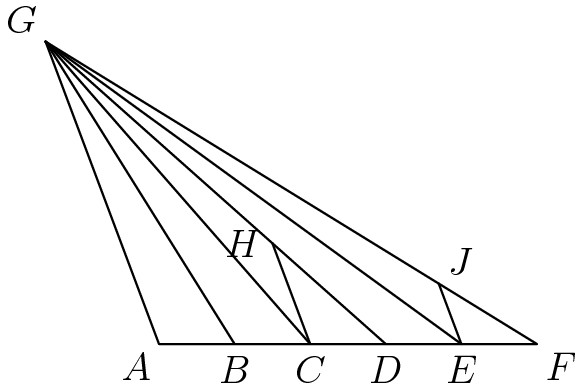
\includegraphics[height=3cm,page=1]{2021-07-17-homework-03}
\end{center}


\fbox{(A) $5/4$ \quad (B) $4/3$ \quad (C) $3/2$ \quad (D) $5/3$ \quad (E) $2$}

\begin{answer}
\begin{align*}
x
\end{align*}
\begin{empheq}[box={\mathbox[colback=white]}]{equation*}
    x
\end{empheq} 
\end{answer}
%%%%%%%%%%%%%%%%%%%%%%%%%%%%%%%%%%%%%%%%%%%%%%%%%%%%%%%%%%%%%%%%%%%%%%%%

\iftoggle{showAnswers}{\newpage}

%%%%%%%%%%%%%%%%%%%%%%%%%%%%%%%%%%%%%%%%%%%%%%%%%%%%%%%%%%%%%%%%%%%%%%%%
\subsection*{4.}

\nopagebreak

In rectangle $ABCD$, $AB = 5$ and $BC = 3$. Points $F$ and $G$ are on $\overline{CD}$ so that $DF = 1$ and $GC = 2$. Lines $AF$ and $BG$ intersect at $E$. Find the area of triangle $AEB$.

\begin{center}
  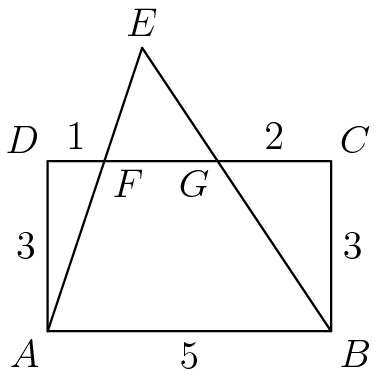
\includegraphics[height=3cm,page=1]{2021-07-17-homework-04}
\end{center}

\fbox{(A) $10$ \quad (B) $\frac{21}{2}$ \quad (C) $12$ \quad (D) $\frac{25}{2}$ \quad (E) $15$}

\begin{answer}
\begin{align*}
x
\end{align*}
\begin{empheq}[box={\mathbox[colback=white]}]{equation*}
    x
\end{empheq} 
\end{answer}
%%%%%%%%%%%%%%%%%%%%%%%%%%%%%%%%%%%%%%%%%%%%%%%%%%%%%%%%%%%%%%%%%%%%%%%%

\iftoggle{showAnswers}{\newpage}

%%%%%%%%%%%%%%%%%%%%%%%%%%%%%%%%%%%%%%%%%%%%%%%%%%%%%%%%%%%%%%%%%%%%%%%%
\subsection*{5.}

\nopagebreak

Points $E$ and $F$ are located on square $ABCD$ so that triangle $BEF$ is equilateral. What is the ratio of the area of triangle $DEF$ to that of triangle $ABE$?

\begin{center}
  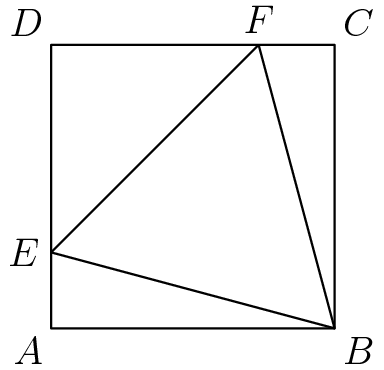
\includegraphics[height=3cm,page=1]{2021-07-17-homework-05}
\end{center}

\fbox{(A) $\frac{4}{3}$ \quad (B) $\frac{3}{2}$ \quad (C) $\sqrt{3}$ \quad (D) $2$ \quad (E) $1+\sqrt{3}$}

\begin{answer}
\begin{align*}
x
\end{align*}
\begin{empheq}[box={\mathbox[colback=white]}]{equation*}
    x
\end{empheq} 
\end{answer}
%%%%%%%%%%%%%%%%%%%%%%%%%%%%%%%%%%%%%%%%%%%%%%%%%%%%%%%%%%%%%%%%%%%%%%%%

\iftoggle{showAnswers}{\newpage}

%%%%%%%%%%%%%%%%%%%%%%%%%%%%%%%%%%%%%%%%%%%%%%%%%%%%%%%%%%%%%%%%%%%%%%%%
\subsection*{6.}

\nopagebreak

In triangle $ABC$ points $D$ and $E$ lie on $\overline{BC}$ and $\overline{AC}$, respectively. If $\overline{AD}$ and $\overline{BE}$ intersect at $T$ so that $AT/DT = 3$ and $BT/ET = 4$, what is $CD/BD$?

\begin{center}
  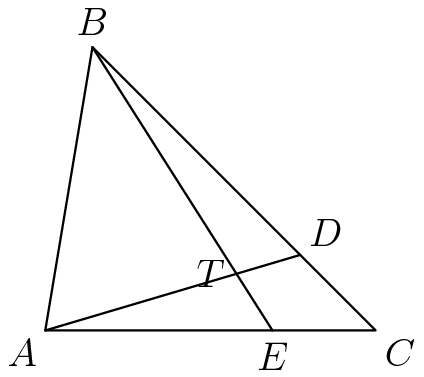
\includegraphics[height=3cm,page=1]{2021-07-17-homework-06}
\end{center}

\fbox{(A) $\frac{1}{8}$ \quad (B) $\frac{2}{9}$ \quad (C) $\frac{3}{10}$ \quad (D) $\frac{4}{11}$ \quad (E) $\frac{5}{12}$}

\begin{answer}
\begin{align*}
x
\end{align*}
\begin{empheq}[box={\mathbox[colback=white]}]{equation*}
    x
\end{empheq} 
\end{answer}
%%%%%%%%%%%%%%%%%%%%%%%%%%%%%%%%%%%%%%%%%%%%%%%%%%%%%%%%%%%%%%%%%%%%%%%%

\iftoggle{showAnswers}{\newpage}

%%%%%%%%%%%%%%%%%%%%%%%%%%%%%%%%%%%%%%%%%%%%%%%%%%%%%%%%%%%%%%%%%%%%%%%%
\subsection*{7.}

\nopagebreak

Triangle $ABC$ has a right angle at $B$, $AB = 1$, and $BC = 2$. The bisector of $\angle BAC$ meets $\overline{BC}$ at $D$. What is $BD$?

\begin{center}
  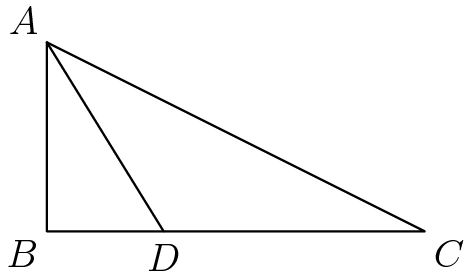
\includegraphics[height=3cm,page=1]{2021-07-17-homework-07}
\end{center}

\fbox{(A) $\frac{\sqrt{3}-1}{2}$ \quad (B) $\frac{\sqrt{5}-1}{2}$ \quad (C) $\frac{\sqrt{5}+1}{2}$ \quad (D) $\frac{\sqrt{6}+\sqrt{2}}{2}$ \quad (E) $2\sqrt{3}-1$}

\begin{answer}
\begin{align*}
x
\end{align*}
\begin{empheq}[box={\mathbox[colback=white]}]{equation*}
    x
\end{empheq} 
\end{answer}
%%%%%%%%%%%%%%%%%%%%%%%%%%%%%%%%%%%%%%%%%%%%%%%%%%%%%%%%%%%%%%%%%%%%%%%%

\iftoggle{showAnswers}{\newpage}

%%%%%%%%%%%%%%%%%%%%%%%%%%%%%%%%%%%%%%%%%%%%%%%%%%%%%%%%%%%%%%%%%%%%%%%%
\subsection*{8.}

\nopagebreak

Right triangle $ABC$ has $AB = 3$, $BC = 4$, and $AC = 5$. Square $XYZW$ is inscribed in triangle $ABC$ with $X$ and $Y$ on $\overline{AC}$, $W$ on $\overline{AB}$, and $Z$ on $\overline{BC}$. What is the side length of the square?

\begin{center}
  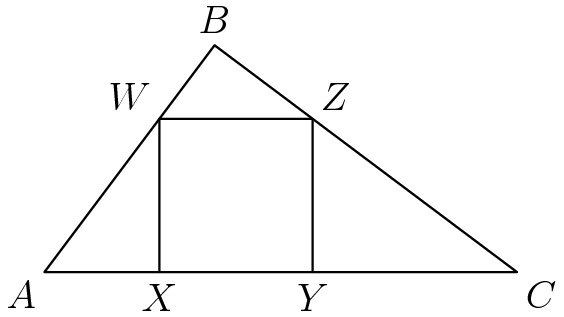
\includegraphics[height=3cm,page=1]{2021-07-17-homework-08}
\end{center}

\fbox{(A) $\frac{3}{2}$ \quad (B) $\frac{60}{37}$ \quad (C) $\frac{12}{7}$ \quad (D) $\frac{23}{13}$ \quad (E) $2$}

\begin{answer}
\begin{align*}
x
\end{align*}
\begin{empheq}[box={\mathbox[colback=white]}]{equation*}
    x
\end{empheq} 
\end{answer}
%%%%%%%%%%%%%%%%%%%%%%%%%%%%%%%%%%%%%%%%%%%%%%%%%%%%%%%%%%%%%%%%%%%%%%%%

\iftoggle{showAnswers}{\newpage}

%%%%%%%%%%%%%%%%%%%%%%%%%%%%%%%%%%%%%%%%%%%%%%%%%%%%%%%%%%%%%%%%%%%%%%%%
\subsection*{9.}

\nopagebreak

A triangle with sides of 5, 12, and 13 has both an inscribed and a circumscribed circle. What is the distance between the centers of those circles?

\fbox{(A) $\frac{3\sqrt{5}}{2}$ \quad (B) $\frac{7}{2}$ \quad (C) $\sqrt{15}$ \quad (D) $\frac{\sqrt{65}}{2}$ \quad (E) $\frac{9}{2}$}

\begin{answer}
\begin{align*}
x
\end{align*}
\begin{empheq}[box={\mathbox[colback=white]}]{equation*}
    x
\end{empheq} 
\end{answer}
%%%%%%%%%%%%%%%%%%%%%%%%%%%%%%%%%%%%%%%%%%%%%%%%%%%%%%%%%%%%%%%%%%%%%%%%

\iftoggle{showAnswers}{\newpage}

%%%%%%%%%%%%%%%%%%%%%%%%%%%%%%%%%%%%%%%%%%%%%%%%%%%%%%%%%%%%%%%%%%%%%%%%
\subsection*{10.}

\nopagebreak

In triangle $ABC$ we have $AB = 25$, $BC = 39$, and $AC = 42$. Points $D$ and $E$ are on $\overline{AB}$ and $\overline{AC}$ respectively, with $AD = 19$ and $AE = 14$. What is the ratio of the area of triangle $ADE$ to the area of the quadrilateral $BCED$?

\fbox{(A) $\frac{266}{1521}$ \quad (B) $\frac{19}{75}$ \quad (C) $\frac{1}{3}$ \quad (D) $\frac{19}{56}$ \quad (E) $1$}

\begin{answer}
\begin{align*}
x
\end{align*}
\begin{empheq}[box={\mathbox[colback=white]}]{equation*}
    x
\end{empheq} 
\end{answer}
%%%%%%%%%%%%%%%%%%%%%%%%%%%%%%%%%%%%%%%%%%%%%%%%%%%%%%%%%%%%%%%%%%%%%%%%

\iftoggle{showAnswers}{\newpage}

\end{document}
